\newpage
\section{Auswertung}

\subsection{Reflexion}

\begin{table}[H]
    \centering
    \begin{tabular}{S [table-format=2.3] S [table-format=2.3]}
        \toprule
        {$\text{Einfallswinkel in Grad}$} & {$\text{Ausfallswinkel in Grad} $}\\
        \midrule
        0.000 & 0.000  \\
        20.000 & 20.000\\
        30.000 & 30.000\\
        40.000 & 40.000\\
        50.000 & 51.000\\
        60.000 & 61.000\\
        70.000 & 70.000\\
        \bottomrule
    \end{tabular}
\caption{Die Messwerte der Reflexion an einem Spiegel}
\label{tab:einf}
\end{table}

\noindent In der Tabelle \ref{tab:einf} sind die Messwerte für dein Einfalls- und den Ausfallswinkel zu finden.\\
Für diese Werte soll das Reflexionsgesetz, $\alpha_1=\alpha_2$, untersucht werden.
Dafür wird auf die Messwerte ein linearer Fit erstellt. 
Dieser hat die Form $f(\alpha)=A \cdot \alpha + B$.\\
Auf die Messwerte gefitet ergibt dies für die Konstanten:
\begin{align*}
    A &= \SI{1.0094(80)}{} \\
    B &= \SI{-0.0779(03570)}{\degree} 
\end{align*}
Grafisch dargestellt findet sich dies in der folgenden Abbildung \ref{img:plot1}.\\



\begin{figure}[h]
    \centering
    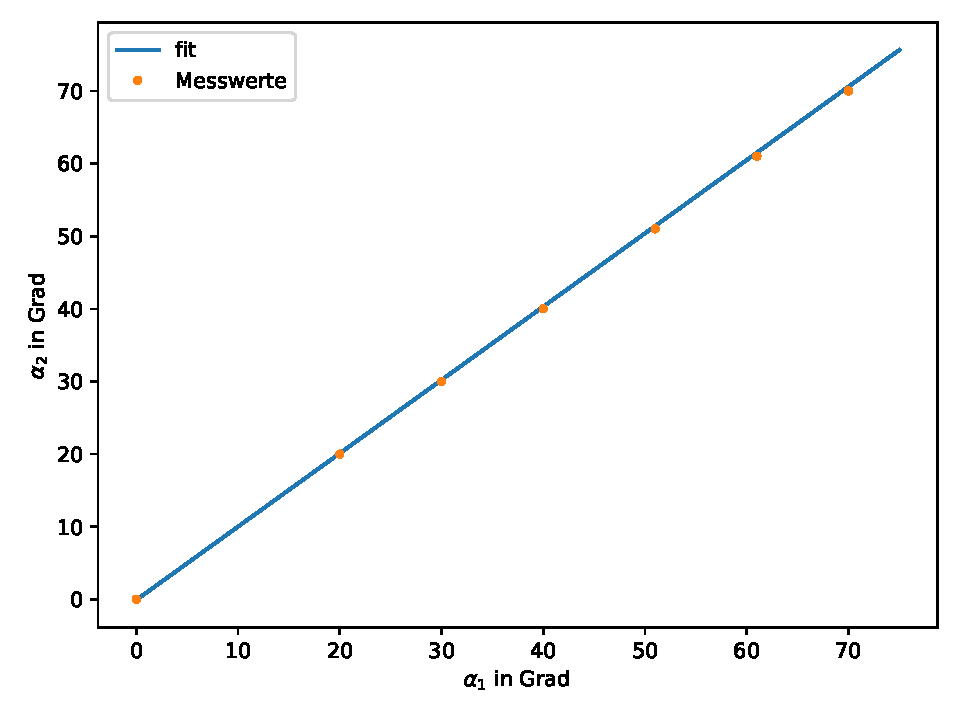
\includegraphics[width=0.6\textwidth]{build/plots/plot1.pdf}
    \caption{Die Messwerte der Reflexion grafisch dargestellt, inklusive Fit-Funktion auf sie.}
    \label{img:plot1}
\end{figure}

\noindent Dieses Ergebnis liegt sehr nah an den Theoriewerten von $A=1$ und $B=0$.\\
Die Idealswerte liegen zwar nicht im Fehlerintervall, für die Steigung ergibt sich aber nach der folgenden Formel folgende relative Abweichung:
\begin{equation*}
    \frac{A_{theo}-A}{A_{theo}}=\SI{-0.9(8)}{\percent}
\end{equation*}

\subsection{Brechung}
\label{sec:sec}


\begin{table}[h]
    \centering
    \begin{tabular}{S [table-format=2.3] S [table-format=2.3] S [table-format=1.3]}
        \toprule
        {$\text{Einfallswinkel in Grad}$} & {$\text{Ausfallswinkel in Grad} $} & {$\text{Brechungsindex} $}\\
        \midrule
        10.000 & 7.000 & 1.425 \\
        20.000 & 14.000 & 1.414\\
        30.000 & 20.000 & 1.462\\
        40.000 & 26.000 & 1.466\\
        50.000 & 31.000 & 1.487\\
        60.000 & 36.000 & 1.473\\
        70.000 & 39.500 & 1.477\\
        \bottomrule
    \end{tabular}
\caption{Die Messwerte der Brehung an Plexiglas. Der Brechungsindex wird dabei aus den Zeilen berechnet.}
\label{tab:brech}
\end{table}

\noindent In Tabelle \ref{tab:brech} sind die für die folgenden Rechnungen genutzten Messwerte zu finden.\\
Die Brechungsindizes in der Tabelle wurden dabei aus den Zeilenwerten mit der folgenden Formel bestimmt:
\begin{equation*}
    n=\frac{\sin(\alpha_1)}{\sin(\alpha_2)}
\end{equation*}
Dabei sind $\alpha_1$ und $\alpha_2$ die Einfalls- und Ausfallswinkel in Bogenmaß umgerechnet.
Wenn nun aus diesen Werten der Mittelwert bestimmt wird und der Fehler des Mittelwerts als Fehler gesetzt 
wird lässt sich der Brechungsindex für Plexiglas zu $n= \SI{1.4578(0105)}{}$ bestimmen.\\
Daraus lässt sich mit der Lichtgeschwindigkeit $c$\cite{c} die Lichtgeschwindigkeit in dem Medium bestimmen.
\begin{align*}
    c_{Plexi}&=c/n \\
    c_{Plexi}&= \SI{205641264.8144 (14778084936)}{\metre\per\second}
\end{align*}
Daraus lässt sich dann auch aus dem Theoriewert für den Brechungsindex $n_{theo}=1.49$\cite{n} auch ein Theoriewert für die Lichtgeschwindigkeit und damit auch die relative Abweichung bestimmen.
\begin{align*}
    c_{theo}&=\SI{201202991.9463}{\metre\per\second}\\
    \frac{c_{theo}-c_{Plexi}}{c_{theo}}&=\SI{-2.2(7)}{\percent}
\end{align*}

\subsection{Parallele Platten}

\begin{figure}[h]
    \centering
    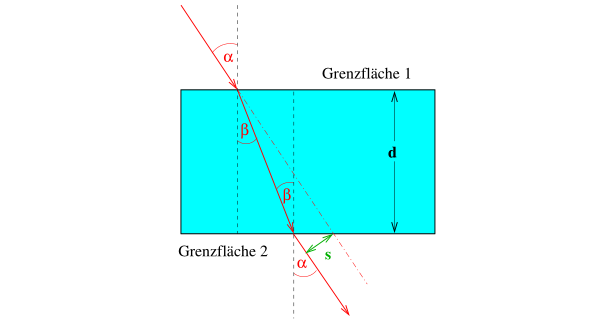
\includegraphics[width=0.6\textwidth]{latex/images/Platten.PNG}
    \caption{Der Durchgang eines Lichtstrahls durch ein Quader eines anderen Mediums.}
    \label{img:platt}
\end{figure}

\noindent Aus der Zeichnung \ref{img:platt} lässt sich ein Gleichung zur Bestimmung des Strahlversatzes $s$ herleiten.\\4
Dafür lässt sich die Hypotenuse $h$ des kleinen Dreiecks, dass mit $s$ aufgespannt wird, durch folgenden Zusammenhang beschreiben:
\begin{equation*}
    h=d\cdot \left( \tan(\alpha)-\tan(\beta)   \right)
\end{equation*}
Hieraus lässt sich dann für $s$ herleiten:
\begin{align*}
    s&=\left( d\cdot \left( \tan(\alpha)-\tan(\beta)   \right) \right) \cdot \cos(\alpha)\\
    s&=d \cdot \left(\sin(\alpha) - \frac{\sin(\beta) \cos(\alpha)}{\cos(\beta)} \right)
\end{align*}
Durch einsetzen der trigonometrischen Identität $\sin(\beta) \cos(\alpha)= -\sin(\alpha-\beta)+\cos(\beta)\sin(\alpha)$ lässt sich das ganze vereinfachen.
\begin{align*}
    s&=d \cdot \left(\sin(\alpha) - \frac{-\sin(\alpha-\beta)+\cos(\beta)\sin(\alpha)}{\cos(\beta)} \right)\\
    s&= d\cdot \frac{\sin(\alpha-\beta)}{\cos(\beta)}
\end{align*}


\noindent Mit dieser Formel und den Werten aus der Tabelle \ref{tab:brech} 
lässt sich damit nun der Strahlversatz berechnen.
Dies wird einmal klassisch, mit den gemessenen Winkeln, und einmal in dem der Winkel $\beta$ mit dem zuvor in \ref{sec:sec} bestimmten Brechungsindex bestimmt wird, gemacht.\\
Die Ergebnisse dieser Rechnung befinden sich, inklusive dem neuen und alten Winkel $\beta$, in der Tabelle \ref{tab:platt}.\\\\

\begin{table}[h]
    \centering
    \sisetup{table-format=1.2}
    \begin{tabular}{S [table-format=1.7]S [table-format=1.7]S [table-format=1.7]S [table-format=1.7]}
        \toprule
        \multicolumn{1}{p{4.2cm}}{\centering$\text{Brechungswinkel klassisch} $\\$ \text{in rad}$} & 
        \multicolumn{1}{p{4cm}}{\centering$\text{Strahlversatz klassisch}$ \\$ \text{in} \si{\metre} $} & 
        \multicolumn{1}{p{3.5cm}}{\centering$\text{Brechungswinkel neu }$\\$ \text{in rad} $} & 
        \multicolumn{1}{p{3.5cm}}{\centering$\text{Strahlversatz neu}$\\$ \text{in} \si{\metre} $ }\\
        \midrule
        0.122173 & 0.000308465 & 0.119397 & 0.00101932 \\
        0.244346 & 0.000630211 & 0.236814 & 0.00210505 \\
        0.349066 & 0.00108104  & 0.35008  & 0.00334175 \\
        0.453786 & 0.0015746   & 0.45662  & 0.00486211 \\
        0.541052 & 0.00222194  & 0.553261 & 0.00691527 \\
        0.628319 & 0.00294111  & 0.636079 & 0.0100675  \\
        0.689405 & 0.00384785  & 0.700471 & 0.0160012  \\
        \bottomrule
    \end{tabular}
\caption{Der Strahlversatz einmal berechnet aus den Messwerten in Tabelle \protect \ref{tab:brech} und einmal in dem der Brechungswinkel neu bestimmt wurde.}
\label{tab:platt}
\end{table}

\noindent Daraus lassen sich nun, wie auch zuvor, folgende Mittelwerte inklusive ihrer Fehler bilden:
\begin{align*}
    s_1&=\SI{0.0018(5)}{\metre}\\
    s_2&=\SI{0.0035(6)}{\metre}\\
    \frac{c_{theo}-c_{Plexi}}{c_{theo}}&\approx\SI{-94.78(6262)}{\percent}
\end{align*} 

\noindent Die relative Abweichung ist hier zwar ziemlich groß, was aber akzeptabel ist da sich in der selben Größenordnung bewegt wird und da der eine Wert sehr viele Fehlerabhängogkeiten besitzt.



\subsection{Prisma}


\begin{table}[h]
    \centering
    \sisetup{table-format=1.3}
    \begin{tabular}{S [table-format=2.3] S [table-format=2.3] S [table-format=1.3]}
        \toprule
        \multicolumn{1}{p{4cm}}{\centering$\text{Einfallswinkel in Grad}$} & 
        \multicolumn{1}{p{4cm}}{\centering$\text{Ausfallswinkel}$ \\ $\text{ des grünen Lasers}$\\$\text{ in Grad} $} & 
        \multicolumn{1}{p{4cm}}{\centering$\text{Ausfallswinkel}$ \\ $\text{ des roten Lasers}$\\$\text{ in Grad} $}\\
        \midrule
        30.000 & 76.500 & 75.000\\
        35.000 & 66.500 & 75.500\\
        40.000 & 58.500 & 57.800\\
        50.000 & 47.000 & 46.000\\
        60.000 & 38.000 & 37.500\\
        \bottomrule
    \end{tabular}
\caption{Die Messwerte der Einfalls- und Ausfallswinkel eines roten und grünen Lasers in einen Prisma.}
\label{tab:prism}
\end{table}

\noindent In Tabelle \ref{tab:prism} sind die gemessenen Werte für den Einfallswinkel zweier Laser in einen Prisma inklusive ihrer Austrittswinkel aufgetragen.
Es handelt sich dabei um einen roten und einen grünen Laser.\\
Im folgenden soll die Ablenkung $\delta$ für die beiden Laser, wie in Abbildung \ref{img:prism} zu sehen, bestimmt werden.
Dafür wird diese Formel genutzt:
\begin{equation*}
    \delta=(\alpha_1+\alpha_2)-(\beta_1-\beta_2)
\end{equation*}
Mit $\gamma=\beta_1+\beta_2$ und $\beta_1=\arcsin(\frac{\sin(\alpha_1)}{n_{kron}})$ lässt sich das ganze noch weiter umformen.\\
Dabei entspricht $\gamma=\SI{90}{\degree}$\cite{V400} und $n_{kron}\approx \SI{1.46}{}$\cite{n}.
\begin{equation*}
    \delta=(\alpha_1+\alpha_2)-(2 \cdot \arcsin(\frac{\sin(\alpha_1)}{n_{kron}}) - \gamma)
\end{equation*}

\begin{figure}[h]
    \centering
    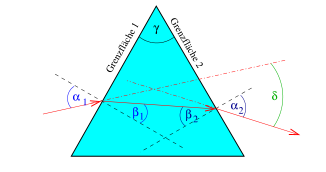
\includegraphics[width=0.5\textwidth]{latex/images/Prisma.PNG}
    \caption{Eine Skizze des Durchgangs von Licht durch einen Prisma.}
    \label{img:prism}
\end{figure}

\noindent
Einsetzten der Werte führt zu folgenden in Tabelle \ref{tab:delta} zu findenden Ergebnissen.

\begin{table}[h]
    \centering
    \begin{tabular}{S [table-format=2.3] S [table-format=2.3] S [table-format=1.3]}
        \toprule
        {$\delta_{gruen}\text{ in Grad}$} & {$\delta_{rot}\text{ in Bogenmaß} $} \\
        \midrule
        2.20689 & 2.18071 \\
        2.01123 & 2.16831 \\
        1.85456 & 1.84234 \\
        1.63547 & 1.61802 \\
        1.48764 & 1.47892 \\
        \bottomrule
    \end{tabular}
\caption{Die Rechenergebnisse für die Ablenkung $\delta$.}
\label{tab:brech}
\end{table}


\noindent Grafisch dargestellt sind diese Werte in Abbildung \ref{img:dunno}.
\begin{figure}[h]
    \centering
    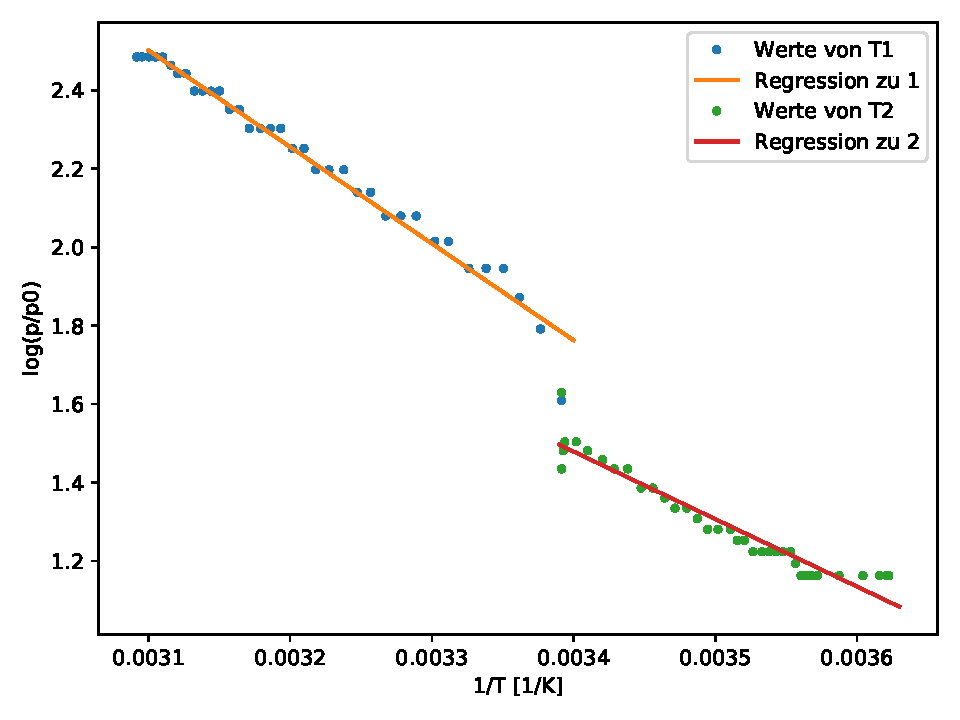
\includegraphics[width=0.5\textwidth]{build/plots/plot2.pdf}
    \caption{Die berechneten Ablenkungen gegen den Ausfallswinkel aufgetragen.}
    \label{img:prism}
\end{figure}


\subsection{Gitter}

\begin{table}[H]
    \centering
    \small
    \sisetup{table-format=1.3}
    \begin{tabular}{S [table-format=1.0]S [table-format=2.3] S [table-format=2.3] S [table-format=1.3]}
        \toprule
        \multicolumn{1}{p{4cm}}{\centering Ordnung\\der\\Maxima} & 
        \multicolumn{1}{p{4cm}}{\centering $d=\SI{1/100}{\milli\metre}$ \\ Winkel des Beugungsmaximums\\ in Grad} & 
        \multicolumn{1}{p{4cm}}{\centering $d=\SI{1/300}{\milli\metre}$ \\ Winkel des Beugungsmaximums\\ in Grad} & 
        \multicolumn{1}{p{4cm}}{\centering $d=\SI{1/600}{\milli\metre}$ \\ Winkel des Beugungsmaximums\\ in Grad}\\
        \midrule
        8&-32.000 &           &         \\
        7&-27.200 &           &         \\
        6&-23.000 &           &         \\
        5&-19.000 &           &         \\
        4&-15.000 &           &         \\
        3&-11.300 &   -35.000 &         \\
        2&-7.500  &   -22.500 &         \\
        1&-4.000  &   -11.000 &-23.500  \\
        0&0.000   &     0.000 &  0.000  \\
        1&3.800   &     11.000& 23.500  \\
        2&7.200   &    22.500 &         \\
        3&11.000  &    35.000 &         \\
        4&15.000  &           &         \\
        5&19.000  &           &         \\
        6&23.000  &           &         \\
        7&27.200  &           &         \\
        8&32.000  &           &         \\
        \bottomrule
    \end{tabular}
\caption{Die Messwerte der Winkel von Begungsmaximas hinter Gittern mit der Gitterkonstante $d$. Zusätzlich ist noch die Ordnung der Maxima abgebildet.\\
Negative Zahlen stehen dabei für die Maxima links vom Maxima 0ter Ordnung. }
\label{tab:git1}
\end{table}

\noindent Die Messwerte der Interferenzmaxima sind in Tabelle \ref{tab:git1} zu finden. 
Zum Weiterrechnen wurde für jede Maximumsordnung das arithmetische Mittel gebildet und die Werte vom 0ten Maxima bereinigt, da dies keine Aussagen über die Wellenlänge der Laser zulässt.
Diese Werte sind in Tabelle \ref{tab:git2} abgebildet.


\noindent Mit Hilfe der folgenden Gleichung, der Ordnung der Beugungsmaxima $k$ und der jeweiligen Gitterkonstante $d$ lässt sich aus den Werten die Wellenlänge $\lambda$ des Lasers bestimmmen:
\begin{equation}
    \lambda = d\cdot \frac{\sin(\phi)}{k}
    \label{eqn:gl}
\end{equation}


\begin{table}[H]
    \centering
    \small
    \sisetup{table-format=1.4}
    \begin{tabular}{S [table-format=1.0]S [table-format=2.3] S [table-format=2.3] S [table-format=1.3]}
        \toprule
        \multicolumn{1}{p{4cm}}{\centering Ordnung\\der\\Maxima} & 
        \multicolumn{1}{p{4cm}}{\centering $d=\SI{1/100}{\milli\metre}$\\ Mittelwert\\ der Beugungsmaximumswinkel\\ in Grad} & 
        \multicolumn{1}{p{4cm}}{\centering $d=\SI{1/300}{\milli\metre}$ \\ Mittelwert\\ der Beugungsmaximumswinkel\\ in Grad} & 
        \multicolumn{1}{p{4cm}}{\centering $d=\SI{1/600}{\milli\metre}$ \\ Mittelwert\\ der Beugungsmaximumswinkel\\ in Grad}\\
        \midrule
        1&3.900   &    11.000 & 23.500  \\
        2&7.350   &    22.500 &         \\
        3&11.150  &     35.000&         \\
        4&15.000  &           &         \\
        5&19.000  &           &         \\
        6&23.000  &           &         \\
        7&27.200  &           &         \\
        8&32.000  &           &         \\
        \bottomrule
    \end{tabular}
\caption{Die Mittelwerte aus Tabelle \ref{tab:git1} inerhalb der Maximumsordnungen gemittelt. }
\label{tab:git2}
\end{table}

\noindent Wenn nun die Werte aus Tabelle \ref{tab:git2} in Gleichung \ref{tab:gl} eingesetzt werden ergeben sich folgende Ergebnisse:

\begin{table}[H]
    \centering
    \small
    \sisetup{table-format=1.3}
    \begin{tabular}{S [table-format=1.0]S [table-format=2.3] S [table-format=2.3] S [table-format=1.3]}
        \toprule
        \multicolumn{1}{p{4cm}}{\centering Ordnung\\der\\Maxima} & 
        \multicolumn{1}{p{4cm}}{\centering $d=\SI{1/100}{\milli\metre}$\\ berechnete Wellenlänge\\ $\si{\pico \metre}$} & 
        \multicolumn{1}{p{4cm}}{\centering $d=\SI{1/300}{\milli\metre}$ \\berechnete Wellenlänge\\ $\si{\pico\metre}$} & 
        \multicolumn{1}{p{4cm}}{\centering $d=\SI{1/600}{\milli\metre}$ \\ berechnete Wellenlänge\\ $\si{\pico\metre}$}\\
        \midrule
        1&  340.076              & 318.015 & 664.582\\
        2&  426.434              & 425.204 &         \\
        3&  483.446              & 191.192 &         \\
        4&  517.638              &          &         \\
        5&  542.614              &          &         \\
        6&  558.187              &          &         \\
        7&  571.372              &          &         \\
        8&  529.919              &          &         \\
        \bottomrule
    \end{tabular}
\caption{Aus den Winkeln der Maxima berechnete Wellenlänge des Lasers.  }
\label{tab:lambda}
\end{table}

\noindent Gemittelt und mit dem Theoriewert von $\lambda= \SI{635}{\pico\metre}$\cite{V400} verglichen ergibt sich folgendes:
\begin{align*}
    \intertext{Für $d=\SI{1/600}{\milli\metre}$:}\\
    \lambda_1&=\SI{664.5818}{\pico\metre}\\
    \symup{Rel_{Abw}}&=\SI{-4.6585}{\percent}\\\\
    \intertext{Für $d=\SI{1/300}{\milli\metre}$:}\\
    \lambda_2&=\SI{885.0468(51437)}{\pico\metre}\\
    \symup{Rel_Abw}&=\SI{39.3774(810030)}{\percent}\\\\
    \intertext{Für $d=\SI{1/100}{\milli\metre}$:}\\
    \lambda_3&=\SI{109.2370(6015887)}{\pico\metre}\\
    \symup{Rel_Abw}&=\SI{-72.0268(947384)}{\percent}
\end{align*}